
%(BEGIN_QUESTION)
% Copyright 2008, Tony R. Kuphaldt, released under the Creative Commons Attribution License (v 1.0)
% This means you may do almost anything with this work of mine, so long as you give me proper credit

When a type ``T'' thermocouple (copper/constantan) is connected to a voltmeter made of copper wires, two active junctions are formed: one at the point of measurement (the measurement junction) and one at a terminal near the voltmeter (the reference junction).  The copper-to-copper junction at the top screw of the terminal block is of no consequence because it is a junction of identical metals, and as such generates no thermoelectric voltage:

$$\includegraphics[width=15.5cm]{i03628x01.eps}$$

The amount of voltage sensed by the voltmeter in this thermocouple circuit is equal to the difference in voltages produced by the measurement and reference junctions:

$$E_{meter} = E_{meas} - E_{ref}$$

\vskip 10pt

Now consider a type ``J'' thermocouple connected to a copper-wire voltmeter.  Here we see there are not two but {\it three} active junctions of dissimilar metals:

$$\includegraphics[width=15.5cm]{i03628x02.eps}$$

Upon first observation it would appear this circuit is more complicated than the type ``T'' thermocouple circuit, owing to the existence of the additional dissimilar-metal junction.  However, a principle called the {\it Law of Intermediate Metals} allows us to consider the two reference junctions (iron-copper and constantan-copper) as electrically equivalent to a single reference junction of iron-constantan, such that the type ``J'' thermocouple circuit becomes just as simple as the type ``T'' circuit with one measurement junction and one reference junction in opposition to each other.

Explain what the {\it Law of Intermediate Metals} is, and how it may be used to simplify the two active reference junctions of the type ``J'' circuit.  Also, explain why it is important that the terminal block be {\it isothermal} in nature.

\underbar{file i03628}
%(END_QUESTION)





%(BEGIN_ANSWER)

The {\it Law of Intermediate Metals} tells us that a series chain of dissimilar metal junctions at the same temperature are electrically equivalent to a single junction comprised of the outer two metals (ignoring all the intermediate metal types between) at that temperature.  Thus, the iron-copper-constantan reference junction pair is electrically equivalent to a single iron-constantan reference junction, so long as both screw terminals are at the same temperature (isothermal).  This principle renders the meter's metal type irrelevant.
 
%(END_ANSWER)





%(BEGIN_NOTES)


%INDEX% Measurement, temperature: thermocouple (law of intermediate metals)

%(END_NOTES)


